
\newpage
\thispagestyle{empty}
\mbox{}
\chapter{Sistema de manera global}
\label{ch:chapter2}

Sea una función $f\left(x\right)$ con $x\in\mathbb{R}^{n}$. Además de ser continua y derivable para todo n. Aplicando el desarrollo en serie de Taylor siendo n = 1.

\begin{equation*}
	f\left(x\right)=f\left(a\right)+f^{'}\left(a\right)\left(x-a\right)+\frac{1}{2!}\cdot{f}^{''}\left(a\right){\left(x-a\right)}^{2}
\end{equation*}

Donde $f^{'}\left(a\right)$ y $f^{''}\left(a\right)$ se corresponden con la primera y segunda derivada de la función en torno a un punto cualquiera en el espacio "$a$", si en lugar de ello se hace con $x_*$, estando x lo suficientemente cerca de dicho punto.

\begin{equation*}
	f\left(x\right)=f\left(x_{*}\right)+f^{'}\left(x_{*}\right)\left(x-x_{*}\right)+\frac{1}{2!}\cdot{f}^{''}\left(x_{*}\right){\left(x-x_{*}\right)}^2 
\end{equation*}

Si $f^{'}\left(x_{*}\right)=0$ se tiene un máximo, mínimo o un punto de inflexión, teniendo esto en cuenta y despejando de la ecuación anterior.

\begin{equation*}
	f\left(x\right)-f\left(x_{*}\right)=\frac{1}{2!}\cdot{f}^{''}\left(x_{*}\right){\left(x-x_{*}\right)}^2 
\end{equation*}

\newpage

Se dan diferentes situaciones:

\begin{itemize}
	\item Si $f^{''}\left(x_{*}\right)<0\rightarrow{f}\left(x\right)-f\left(x_{*}\right)<0\rightarrow{f}\left(x\right)<f\left(x_{*}\right)\rightarrow{f}\left(x_{*}\right)$ es un máximo.
	\item Si $f^{''}\left(x_{*}\right)>0\rightarrow{f}\left(x\right)-f\left(x_{*}\right)>0\rightarrow{f}\left(x\right)>f\left(x_{*}\right)\rightarrow{f}\left(x_{*}\right)$ es un mínimo.
	\item Si $f^{''}\left(x_{*}\right)=0\rightarrow{f}\left(x\right)-f\left(x_{*}\right)=0\rightarrow{f}\left(x\right)=f\left(x_{*}\right)\rightarrow{f}\left(x_{*}\right)$ es un punto de inflexión.
\end{itemize}

Si se hace el mismo desarrollo y se expande el dominio para $n\geq{2}$, se obtiene:

\begin{equation}\label{TaylorNormal}
	f\left(x\right)=f\left(x_{*}\right)+\mathrm{\nabla}{f}{\left(x_{*}\right)}^{T}\left(x-x_{*}\right)+\frac{1}{2!}\cdot{\left(x-x_{*}\right)}^{T}\cdot{H}\left({f}\left(x_{*}\right)\right) 		\cdot\left(x-x_{*}\right)
\end{equation}

Donde:

\begin{equation*}
	\begin{aligned}
		\mathrm{\nabla}{f}=
	\begin{bmatrix}
		\frac{\partial{f}}{\partial{x}_1} \\
		\frac{\partial{f}}{\partial{x}_2}  \\
		\vdots \\
		\frac{\partial{f}}{\partial{x}_n}
	\end{bmatrix}
	\end{aligned}
	\qquad\text{y}\qquad
	\begin{aligned}
	{H}\left(f\right)=\mathrm{\nabla}^{2}{f}= 	
	\begin{bmatrix}
		\frac{\partial^{2}{f}}{\partial{x}_{1}^{2}} & \frac{\partial^{2}{f}}{\partial{x}_{1}\cdot\partial{x}_{2}} & \cdots & \frac{\partial^{2}{f}}{\partial{x}_{1}\cdot\partial{x}_{n}}\\
		\frac{\partial^{2}{f}}{\partial{x}_{2}\cdot\partial{x}_{1}} & \frac{\partial^{2}{f}}{\partial{x}_{2}^{2}} & \cdots & \frac{\partial^{2}{f}}{\partial{x}_{2}\cdot\partial{x}_{n}}\\
		\vdots & \vdots & \ddots & \vdots\\
		\frac{\partial^{2}{f}}{\partial{x}_{n}\cdot\partial{x}_{1}} & \frac{\partial^{2}{f}}{\partial{x}_{n}\cdot\partial{x}_{2}} & \cdots & \frac{\partial^{2}{f}}{\partial{x}_{n}^{2}}
	\end{bmatrix}
	\end{aligned}
\end{equation*}\\

En este caso lo que interesa es que el gradiente de la función sea 0, es decir, que "$\mathrm{\nabla}{f}{\left(x_{*}\right)}=0$". Por lo tanto, los casos particulares previamente descritos adoptan un significado similar. 

\begin{equation*}
	f\left(x\right)-f\left(x_{*}\right)=\frac{1}{2!}\cdot{H}\left(f\right)\cdot\left(x-x_{*}\right)^2 
\end{equation*}

\begin{itemize}
	\item Si ${H}\left(f\right)<0$ (definida negativa) $\rightarrow{f}\left(x\right)-f\left(x_{*}\right)<0\rightarrow{f}\left(x_{*}\right)$ es un máximo.
	\item Si ${H}\left(f\right)>0$ (definida positiva) $\rightarrow{f}\left(x\right)-f\left(x_{*}\right)>0\rightarrow{f}\left(x_{*}\right)$ es un mínimo.
	\item Si ${H}\left(f\right)=0$ es indefinida es un punto silla.
\end{itemize}

En caso de las funciones para dos o más dimensiones, la condición necesaria para ser optimo es estar semidefinido, es decir, si $\mathrm{\nabla}{f}{\left(x_{*}\right)}=0$ y ${H}\left(f\right)$ es semidefinida, se tiene:

\begin{itemize}
	\item Es máximo si esta semidefinida negativa $\rightarrow{y}^{T}\cdot{H}\left({f}\right)\cdot{y}\leq{0}$
	\item Es mínimo si esta semidefinida positiva $\rightarrow{y}^{T}\cdot{H}\left({f}\right)\cdot{y}\geq{0}$
\end{itemize}

\section{Algoritmo de estimación del gradiente/de busqueda de fuentes (decidir luego}


\subsection{Descripción general}

Se pretende describir un procedimiento para la búsqueda de fuentes mediante la estimación del gradiente de una función $\widehat{\mathrm{\nabla }}{f}\left(c\right)$, basándose en mediciones locales de múltiples robots situados de manera simétrica en un espacio de 2D. En dicho procedimiento, se consideran N robots distribuidos uniformemente a lo largo de una formación circular con un radio D y un punto central c definido en dos dimensiones. [poner referencia]

Partiendo de la ecuación \ref{TaylorNormal} pero haciendo la expansión únicamente hasta el termino de primer orden sobre cada una de las medidas $r_i$ pertenecientes a la función ${f}\left({r}_{i}\right)$ y despejando el gradiente se llega a:

\begin{equation*}
	\frac{2}{{D}^2\cdot{N}}\cdot\sum_{i=1}^{N}f(r_{i})\cdot(r_{i}-c)=\underbrace{\nabla{f}\left(c\right) + \varphi\left(D,c\right)}_{:=\hat{\nabla}{f}\left(c\right)}
\end{equation*}

Donde se tiene un termino de error $\varphi\left(D,c\right)$ que va a corresponder al remanente de orden 2 de la expasión de Taylor..

Para dicho calculo, adopta vital importancia los \textbf{algoritmos de tipo consenso} siendo estos un mecanismo que permite a maquinas coordinarse en un entorno distribuido, es decir, encuentran la solución al problema de la comunicación entre diferentes entes aislados con el objetivo de ponerse de acuerdo para realizar una tarea concreta.

Adicionalmente, las funciones sobre las que se basa el algoritmo han de cumplir ser \textbf{lipzchiana} cuya definición se describe a continuación. Posterior a ello, en el capitulo 3 se dará un desarrollo más profundo del algoritmo, en donde, se verá toda la base matemática sobre la que se sustenta.

\subsection{Función lipzchiana}

Dada una función $f:\mathnormal{U}\subset\mathbb{R}^{n}\rightarrow\mathbb{R}^{m}$, se dice que $f$ es globalmente Lipschitz en el conjunto $\mathnormal{U}$ cuando existe una constante $L>{0}$ tal que 

\begin{equation*}
	|f\left(x\right)-f\left(y\right)|\leq\mathnormal{L}|x-y|\Longleftrightarrow\mathnormal{L}\geq|f^{'}\left(x\right)|\hspace{10mm}\forall_{x,y}\in\mathnormal{U} [referencia bibliografica]
\end{equation*}

La importancia de uso de dicho tipo de función recae en el criterio de convergencia utilizado por el algoritmo, es decir, se garantiza que siempre y cuando la función sobre la que se desplazan los agentes sea lipzchiana estos van a llegar de manera exitosa al punto de interés.\\

\begin{figure}[htb]
  \begin{center}
    \subfigure[Función definida en 3D]{
        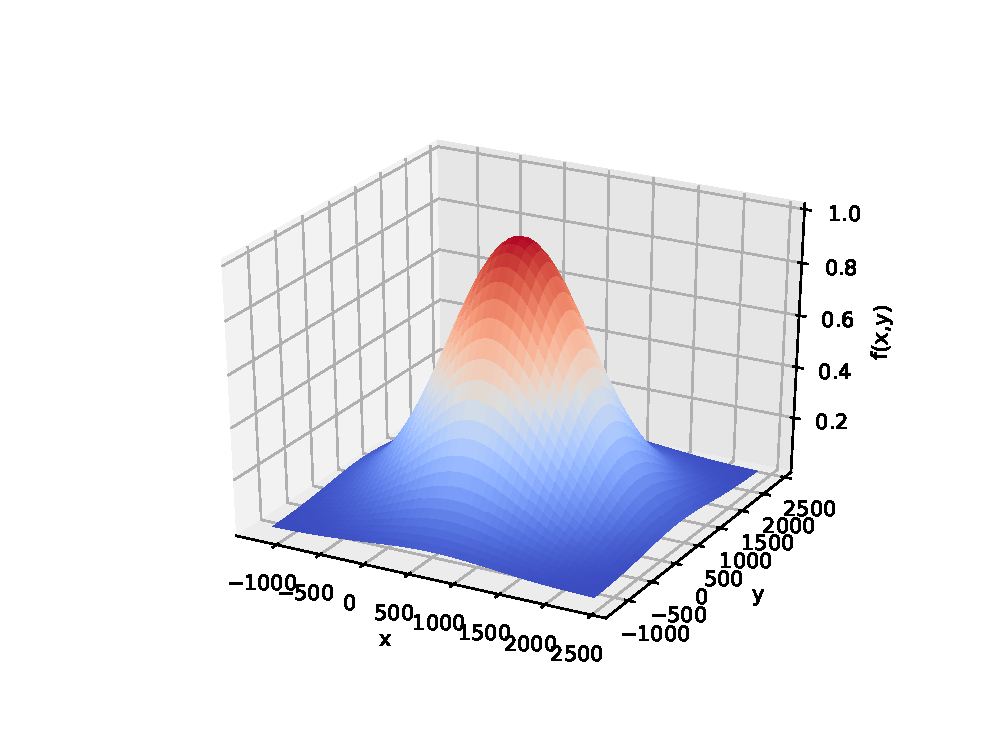
\includegraphics[width=0.45\textwidth]{figures/Gaussiana.eps}
        \label{Fgauss}}
    \subfigure[Curvas de nivel]{
        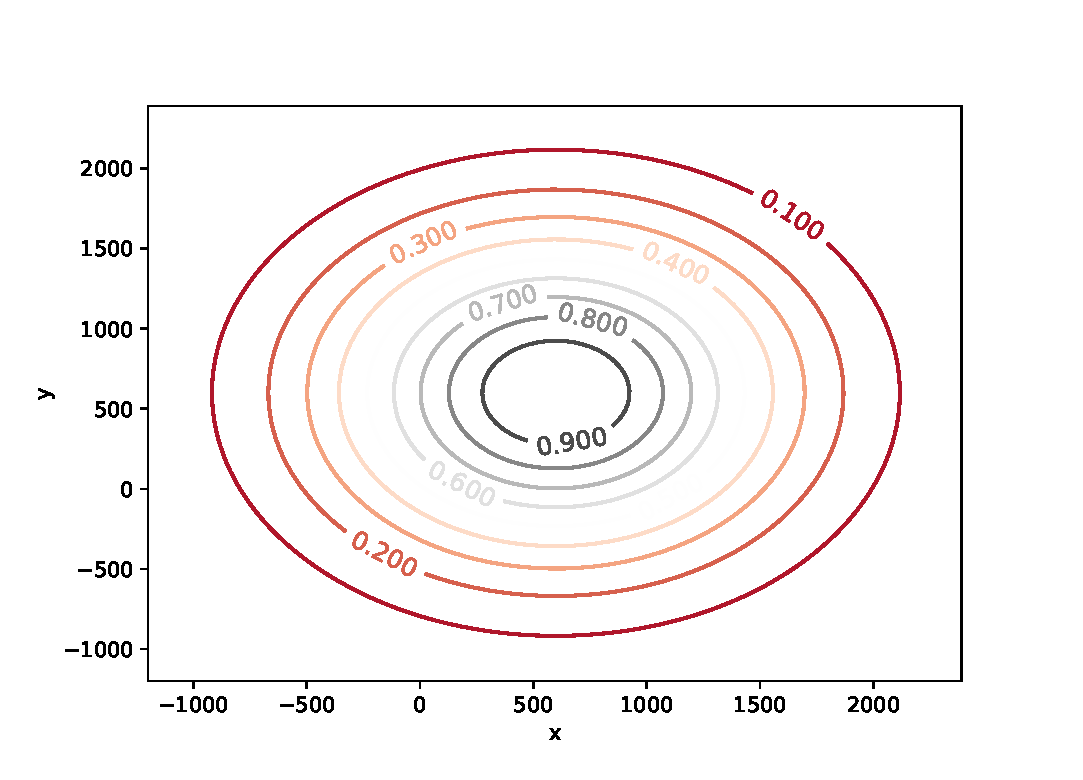
\includegraphics[width=0.45\textwidth]{figures/CurvasNivelGauss.eps}
        \label{CurvasGauss}}
    \caption{Representación de una función lipzchiana}
    \label{FunGauss}
  \end{center}
\end{figure}

Se destaca que toda función lipzchiana a su vez debe ser cuadrática. No obstante, toda función cuadrático no es lipzchiana, un ejemplo de ello es $x^2 = 0$ la cual no esta acotada en un intervalo de la recta. Por ello, se propone la utilización de distribuciones gaussianas para evaluar la eficacia del algoritmo.

Por ende, se define una distribución gaussiana de la siguiente forma:

\begin{equation*}
	f\left(x,y\right)=k·e^{-H}\hspace{10mm}con\hspace{2mm}H=P·S·P^{T}
\end{equation*}

Donde $P=\left[x,y\right]$ son sus coordenadas definidas $\forall_{x,y}\in\mathbb{R}$ y $S=\left[S_x,S_y\right]$ es su desviación siendo una matriz cuadrada y diagonal que mientras más grande sean sus valores más plana será y consecuentemente sus curvas de nivel cubrirán un espacio más amplio, además, su centro va a estar definido como $c=\left[c_x,c_y\right]$.

Finalmente, para la simulación del algoritmo se propuso situar el centro en $c=\left[600,600\right]$, tener una desviación $S=\left[\frac{1000}{sqrt{2}},\frac{1000}{sqrt{2}}\right]$ y finalmente un valor de $k=1$ tal como puede apreciarse en la figura \ref{FunGauss}.

\section{Algoritmo de control de formación circular}

\subsection{Control de formación}

El control de la formación tiene como objetivo evaluar la cooperación y la coordinación en sistemas con múltiples agente, donde su uso recae en impulsarlos a lograr unas restricciones prescritas en sus estados conllevando a formar y mantener una forma geométrica deseada.

Las características esenciales de este tipo de control están relacionadas con la capacidad de detección y la topología de interacción de la red formada por los agentes. Esto conlleva a diferenciar dos tipos de variables:

\begin{itemize}
	\item \textbf{Detectadas:} Especifican la capacidad de detección de los agentes individuales, un ejemplo de ello sería la velocidad u orientación que posee cada agente.
	\item \textbf{Controladas:} Son aquellas relacionadas con la topología de interacción, es decir, sirve para detallar la mejor formación deseada posible que puedan lograr los agentes.
\end{itemize}

\subsection{Descripción general del algoritmo}

El problema de control considera vehículos tipo monociclo con velocidad constante, es decir, solo se actúa sobre la dirección del vehículo a través de giros coordinados actuando sobre el ángulo de inclinación lateral de la aeronave. A esto se le añade la velocidad del viento que altera la velocidad constante propia llevaba por cada agente cuyo marco de coordenadas se encuentra fijado en el centro de una formación circular. Sin embargo, se asumirá que la velocidad del viento es mucho menor que la velocidad deseada, por lo que la velocidad respecto al suelo puede considerarse casi constante durante la misión del vehículo. [2].

El objetivo es describir u  \textbf{algoritmo distribuido para controlar formaciones circulares} de UAV de ala fija con velocidades constantes que actúa sobre el radio del circulo a ser rastreado no sobre la dirección de cada uno de los agentes, es decir, altera la velocidad angular que poseen en torno a un punto central (centro de la circunferencia).\\

\begin{figure}[htb]
\centering
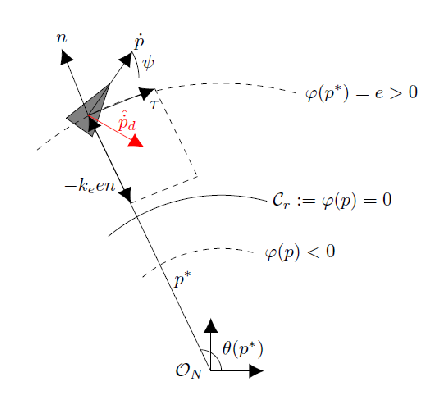
\includegraphics[width=0.6\textwidth]{figures/TA.eps}
\caption{Trayectoria descrita por cada uno de los agentes [Referencia bibliográfica]} \label{fig:Trayectory}
\end{figure}

En resumidas cuentas, cada uno de los robots se encontrarán en un punto $p^*$ cualquiera y ha de converger a un centro definido $C_r$, donde $p^* \cap {C}_r \in \mathbb{R}^{2}$. Consecuentemente, mediante la siguiente ecuación se puede describir los comportamientos adoptados por los agentes.

\begin{equation}\label{Control}
	\varphi\left(p\right)=c_i \Longrightarrow x^2+y^2 - r^2 = c_i
\end{equation}

En donde, $c_i \in \mathbb{R}$ siendo la señal de control que se diseñará y el superindice $i$ denota cada uno de los vehículos/agentes/robots (ver que poner). Se definen dos casos particulares:

\begin{itemize}
	\item Si $c_i$ se hace muy pequeño, el radio tenderá a aumentar y con ello se reduce la velocidad angular.
	\item Si $c_i$ se hace muy grande, el radio tenderá a disminuir y con ello se aumenta la velocidad angular.
\end{itemize}

Ambos casos tienen como objetivo converger a la formación circular definida previamente. Finalmente, en esta sección únicamente se trato al algoritmo de manera simplificada dado que más adelante, en el capitulo 4, se dará una descripción más detallada de este, en donde se verán dos formas de consenso entre los agentes, el comportamiento propio descrito para cada uno de ellos o el criterio de convergencia de los agentes.

\section{Acción conjunta de ambos algoritmos}

\subsection{Algoritmo de ascenso de gradiente}

Hasta el momento únicamente se ha comentado sobre la cooperación de los agentes para la disposición de una figura geométrica y simétrica requerida o un algoritmo para la localización de fuentes en el espacio. No obstante, se ha dejado de lado el avance de los agentes, es decir, ha de existir un algoritmo que desplace a todo el enjambre hacia la ubicación de la fuente haciendo uso del gradiente estimado.

Para ello, se utiliza el algoritmo de ascenso de gradiente para desplazar el centro de la formación circular, el cual se encuentra definido de la siguiente forma:

\begin{equation}\label{GA}
	c_{k+1}=c_k+\epsilon\nabla{f}\left(c_k\right)\hspace{10mm}[Referencia bibliografica]
\end{equation}

En donde, $c_k=[x,y]\hspace{2mm}\forall_{x,y}\in\mathbb{R}$ siendo este el centro de la formación circular. Al tratarse de un problema definido como un punto máximo de una función, el avance ha de ser estrictamente positivo, es decir, los valores han de ser cada vez mayores para desplazarte hacia dicho punto. Esto es debido al valor que toma la función siendo $\rightarrow{f}\left(c_k\right)-f\left(c_{k*}\right)<0\rightarrow{f}\left(c_{k*}\right)$ con $\mathrm{\nabla}{f}{\left(c_{k*}\right)}=0$ tal como se vio al inicio del capitulo.

\subsection{Dinámica del sistema}


\begin{figure}[htb]
\centering
\includegraphics[width=0.6\textwidth]{figures/Flujo2.eps}
\caption{Diagrama de flujo que describe la dinámica del sistema [Referencia bibliográfica]} \label{fig:Flujo}
\end{figure}

En la figura \ref{fig:Flujo} se pueden apreciar diferentes colores para diferenciar cada uno de los pasos a seguir antes de llegar a la fuente final, desglosándolos estos serían:

\begin{enumerate}
	\item Se disponen los N agentes en el plano.
	\item Se ejecuta el algoritmo de control de formación circular que cuando los agentes estén dispuestos de manera simétrica, es decir, sus posiciones absolutas no alteren mucho el resultado de la estima del gradiente pasará a la siguiente fase, en caso contrario se quedará esperando que se coloquen en sus sitios.
	\item Al ya estar repartidos alrededor de la formación circular, se hace la estimación del gradiente para obtener la localización de la fuente. En este punto, se dan dos casos que en la figura \ref{fig:Flujo} están referidos como A:
	\begin{itemize}
		\item Si $\widehat{\mathrm{\nabla }}{f}\left(c_{k}\right)\approxeq0$ se está cerca de la fuente conformando una \textbf{solución satisfactoria}.
		\item Si $\widehat{\mathrm{\nabla }}{f}\left(c_{k}\right)>0$ aun están desplazándose para llegar al objetivo.
	\end{itemize}
	\item Si se da la segunda de las situaciones antes planteadas, se ha de desplazar el centro de la formación circular mediante el algoritmo de ascenso de gradiente, tal como se vio en el apartado [hacer referencia al capitulo anterior].
	\item Antes de volver a estimar el gradiente se debe comprobar el paso 2, en caso de permanecer en sus posiciones de la formación directamente partes del paso 3.
\end{enumerate}



